\documentclass[11pt,a4paper]{article}
\usepackage[T1]{fontenc}
\usepackage[utf8]{inputenc}
\usepackage{lmodern,microtype}
\usepackage{cite}
\usepackage{needspace}
\usepackage[section]{placeins}
\usepackage[margin=22mm,headheight=14pt]{geometry}
\usepackage{graphicx,booktabs,tabularx,array,amsmath,enumitem,float}
\usepackage{xcolor,tikz,caption,fancyhdr,titlesec}
\usetikzlibrary{arrows.meta,positioning,fit,calc}
\definecolor{navy}{HTML}{183850}
\definecolor{lightblue}{HTML}{EDF3F7}
\definecolor{muted}{HTML}{526575}
\usepackage[colorlinks=true,linkcolor=navy,citecolor=navy,urlcolor=navy]{hyperref}
\hypersetup{pdftitle={Exploring New Information Visualization Techniques for VisuAlgo+ (CP4101 CA Report)},pdfauthor={Truong Van Quoc Bao}}
\setlength{\parindent}{0pt}
\setlength{\parskip}{6pt}
\linespread{1.06}
\setlist{nosep,leftmargin=1.6em}
\setlength{\emergencystretch}{2em}
\renewcommand{\arraystretch}{1.18}
\titleformat{\section}{\Large\bfseries\color{navy}}{\thesection}{.65em}{}
\titleformat{\subsection}{\large\bfseries\color{navy}}{\thesubsection}{.65em}{}
\titlespacing*{\section}{0pt}{0pt}{10pt}
\titlespacing*{\subsection}{0pt}{12pt}{4pt}
\captionsetup{font=small,labelfont=bf,skip=5pt}
\pagestyle{fancy}\fancyhf{}
\fancyhead[L]{\small\color{muted}VisuAlgo+}
\fancyhead[R]{\small\color{muted}CP4101 CA Report \textbar\ H160390}
\fancyfoot[C]{\small\thepage}
\renewcommand{\headrulewidth}{.3pt}
\newcommand{\code}[1]{\texttt{#1}}
\newcommand{\shot}[4]{\begin{figure}[tbp]\centering\includegraphics[width=#2\linewidth]{figures/#1}\caption{#3}\label{#4}\end{figure}}
\newcommand{\page}{\par\Needspace{5\baselineskip}\vspace{6pt}}
\renewcommand{\topfraction}{.85}\renewcommand{\bottomfraction}{.6}\renewcommand{\textfraction}{.12}\renewcommand{\floatpagefraction}{.75}\setcounter{topnumber}{3}\setcounter{totalnumber}{4}
\begin{document}
\begin{titlepage}
\centering
{\large NATIONAL UNIVERSITY OF SINGAPORE\\School of Computing\par}
\vspace{16mm}
{\LARGE\bfseries\color{navy}Exploring New Information Visualization\\Techniques for VisuAlgo+\par}
\vspace{4mm}
{\large Rebuilding Interactive Algorithm Visualizations\par}
\vspace{9mm}
{\Large CP4101 Final Year Project\\Continuous Assessment Report\par}
\vspace{10mm}
{\large Truong Van Quoc Bao\\A0276275U\par}
\vspace{6mm}
{Project ID: H160390\\Supervisor: A/P Steven Halim\\Main Evaluator: SIM Mong Cheng, Terence\\Academic Year 2026/27, Semester 1\\4 November 2026\par}
\vspace{9mm}
\begin{minipage}{.94\textwidth}
\textbf{Abstract.} VisuAlgo+ is a collaborative project to rebuild VisuAlgo with a renewed technical foundation and a redesigned interface while preserving its educational purpose. My work focuses on the visualization and interaction layer: graph, tree and sorting visualizers, their editing and playback behaviour, and their integration into a common interface. The work began with standalone prototypes and progressed to a single application using a shared panel layout. This report explains the separation of input, layout and playback state; a shared panel-group layout (V10); algorithm extensions and their validation; and floating text, short explanations placed on the drawing. The current application contains 11 graph algorithms (counting the two DFS variants separately), seven tree workspaces and eight sorting algorithms. Its recorded validation on 1 November 2026 reports 3,273 passing unit tests and 151 passing browser cases. These results support functional progress. A formative user trial in Week 10 informed several UI/UX refinements, including floating text and adjustments to the legend and Status panel. Neither the tests nor the trial establishes improved learning outcomes or comparative usability. In Semester 2, the visualizers will be merged with the shared infrastructure into one complete web application, alongside stronger interaction testing and an evaluation with representative learning tasks.
\end{minipage}
\end{titlepage}
\setcounter{page}{2}

\begingroup
\setlength{\parskip}{4pt}
\linespread{1.0}\selectfont
\section{Introduction and Objectives}
\subsection{Project background}
VisuAlgo provides interactive visualizations of data structures and algorithms. Its original design brings different topics into a consistent environment and allows students to explore their own inputs~\cite{halim2012}. These strengths are the starting point for VisuAlgo+.

In an early discussion, A/P Steven Halim described the existing Laravel/PHP, MySQL, D3 and jQuery stack. Some of these tools have become dated and no longer suit the planned future updates, so his aim for this version is to use the best currently available tools for both the interface and the execution engine. The rebuild still retains useful technologies, including D3 for selected layout and animation tasks.

The aim is a modern successor that preserves VisuAlgo's educational purpose and useful interactions while supporting future development. The current deliverable is an experimental application, not yet a full replacement.

\subsection{Personal motivation and role}
My motivation for joining VisuAlgo+ comes from my background in competitive programming and teaching. Participating in many programming competitions and achieving strong results has given me substantial experience with algorithms and data structures. Teaching students passionate about competitive programming has helped me explain these concepts from different perspectives and recognize where learners need clarification.

I hope to apply both experiences to VisuAlgo+'s user interface and user experience (UI/UX), helping learners follow why an algorithm makes a decision, how its state changes, and how those changes produce the result. This perspective guides which intermediate states I show, how I connect drawings with pseudocode, and where short explanations could clarify a step.

My initial responsibility is the visualization and interaction layer for graph algorithms, tree-based data structures and sorting algorithms. This includes developing the visualizers, supporting input editing and step-by-step playback, and integrating them into a consistent interface. Working with Kerk Tai Heng, a fellow FYP student, on the shared design and integration, I aim to turn my algorithmic knowledge and teaching experience into practical improvements that can later be evaluated with learners.

\subsection{Objectives and current scope}
The project has five working objectives:
\begin{enumerate}
\item Select suitable modern and widely adopted technologies for rebuilding the platform.
\item Preserve useful algorithm exploration, input editing and step-by-step explanation from VisuAlgo.
\item Provide a consistent interface across different algorithm and data-structure modules.
\item Establish clear boundaries for extending visualizers and integrating execution engines.
\item Validate the rebuilt functionality and identify what still requires technical and user evaluation.
\end{enumerate}

Kerk, who has the same supervisor, works on the WebAssembly engine foundation, website design system and shared infrastructure. Section~\ref{sec:approach} details our contributions and collaboration.

The current application targets desktop and laptop use. It runs TypeScript algorithm implementations in the browser. The separate WebAssembly engine has not been connected to these visualizers. Mobile design, complete feature parity with VisuAlgo and measured learning improvement are outside the completed work reported here.

\endgroup
\page
\section{Background and Related Work}
\subsection{Algorithm visualization and educational use}
Halim et al.~\cite{halim2012} present the unified, interactive web-based environment for learning algorithms that later became VisuAlgo. Support for user-defined inputs and consistent interaction across topics is particularly relevant to this project. A reconstruction should preserve these properties even when the rendering technology and page layout change. Reusing familiar examples and algorithm operations also provides a useful reference when checking the rebuilt functionality.

However, a working animation is not sufficient evidence of learning benefit. Hundhausen, Douglas and Stasko's meta-study of 24 studies~\cite{hundhausen2002} found that how learners used algorithm visualizations mattered more than their graphical characteristics alone. This motivates a distinction between two questions in VisuAlgo+: whether the software behaves correctly, and whether students can use it to understand and explain an algorithm. The present tests primarily address the first question; the Week 10 trial (Section~\ref{sec:trial}) gave formative input on the second, and a structured follow-up is planned.

OpenDSA combines visualizations with explanatory material, interactive exercises and proficiency assessment~\cite{opendsa}. It illustrates how visualization can form one part of a wider learning activity. VisuAlgo+ currently concentrates on exploration: editing inputs, stepping through execution, following pseudocode and inspecting state. It does not yet provide an equivalent assessed learning sequence. Therefore, the current contribution should be judged as a visualization foundation rather than a complete instructional system.

\subsection{Reusable platforms and implementation choices}
Shaffer et al.~\cite{shaffer2010} survey the algorithm-visualization field and discuss issues including availability, quality and topic coverage. Their survey motivates attention to maintainable implementations and reusable interaction patterns.

For the technical foundation, React Flow supplies an interactive node-and-edge canvas~\cite{reactflow}. The project builds algorithm-specific state, edge identities and presentation rules above that canvas. D3 supplies narrower computational tools: force simulation for graph positions and a hierarchy layout for trees~\cite{d3}. This combination separates the computation of positions from the ownership of application state. Sorting uses Canvas 2D because its main representation is an array of bars rather than an editable graph.

\subsection{Position of this work}
The project applies established algorithm, rendering and interface ideas to a practical rebuild. Its current value lies in connecting them coherently: a stable editable document, reproducible playback, shared page controls, and explanations tied to individual algorithm steps. Dockable panels and low-link algorithms are not claimed as new research techniques.

Three design questions guide the work. First, how can editing and playback share one canvas without accidentally invalidating or corrupting an execution? Second, how can different topics share a layout while preserving their own interactions? Third, how can a step remain understandable when it changes internal state but produces little visible motion? Sections~\ref{sec:state}--\ref{sec:notes} describe the implemented responses.

\page
\section{Development Approach and Responsibilities}\label{sec:approach}
\subsection{From standalone prototypes to one application}
The first stage, starting before the semester, explored interaction behaviour in standalone repositories. The first graph prototype has its first recorded commit on 28 July 2026; a second graph prototype followed in August with a clearer separation of document, layout and playback state. Sorting and tree prototypes explored different representations and operation models. This work provided a functional base before integration with the shared website.

During September and October, I adapted these visualizers to Kerk's design system. Kerk's wireframe of the visualization page drew nine candidate layouts, numbered V1--V9. After a user survey organized by Kerk, Kerk and I chose two of them, V2 (split rails) and V7 (docks), and I built the graph, tree and sorting visualizers in both layouts with comparable functionality (20--27 September). In Week 9, Kerk and I discussed a proposal to combine V2 and V7 into a tenth layout, V10, retaining selected strengths of each. I implemented V10, and Kerk contributed refinements to complete the version later used in the Week 10 trial. The survey served as formative input only; its responses are not analysed in this report.

On 18 October, Kerk consolidated the separate site and visualizer copies into one application and moved common code into a shared layer. Kerk and I then ran a separate formative user trial in Week 10 (Section~\ref{sec:trial}). Subsequent work extended algorithms, added floating text and resolved defects found in review. Table~\ref{tab:timeline} summarizes these stages.

\begin{table}[tbp]\small\centering
\caption{Main development stages.}\label{tab:timeline}
\begin{tabularx}{\linewidth}{@{}>{\raggedright\arraybackslash}p{24mm}X@{}}\toprule
Period & Main outcome\\\midrule
July--August & First graph prototype (first recorded commit 28 July, before the semester); second graph prototype with separated document, layout and playback state; standalone sorting prototype.\\
September & Tree workspaces; adaptation to Kerk's design system; V2 and V7 layouts built (20--27 Sept.); unmerged experiment on Kerk's engine.\\
29 Sept.--17 Oct. & Recursive DFS, Bellman--Ford and Prim; lazy segment tree and AVL deletion; playback refinements; V10 discussed (Week 9) and implemented.\\
18--31 Oct. & One-app consolidation (Kerk); LCA and heap operations; Week 10 user trial; topological sort, bipartite check, cut vertices and bridges; floating text; review fixes.\\
1--4 Nov. & Recorded validation (1 November) and report preparation.\\\bottomrule
\end{tabularx}
\end{table}

\subsection{Individual contribution and collaboration}
My principal contributions are the standalone visualizer foundations and their integration, including the site's homepage, routing and host boundary (built on Kerk's design system) and the Graph and Tree Editors; the core V10 layout model; algorithm and operation extensions; and the shared floating-text layer, together with most of their automated tests and design-decision records. Of the 48 numbered design choices in the V10 proposal, the first 26 were my decisions. Choices 27--48 (18--22 October) and the 18 October decision to keep only V10 were made by Kerk and me together and implemented by Kerk. Kerk also owns the original design system, engine foundation, infrastructure and application consolidation. These responsibilities overlap at integration boundaries~\cite{evidence}. From Week 8, Kerk and I drafted a plan for the remaining work, which our supervisor reviewed and agreed to: Semester 1 completes and tests the prototypes, and Semester 2 merges them into one complete web application, which requires integrating the shared infrastructure (Section~\ref{sec:plan}).

I used Claude and Codex for implementation, debugging, test generation and review under my requirements and design choices. My acceptance workflow included reading changes, running the application and using tests or continuous integration (CI) results. In late-October review sessions, Codex identified findings, Claude reproduced findings, and I selected the fixes to pursue. AI also assisted in organizing evidence and drafting this report. Such assistance is part of the development process; generated code and passing tests still require critical review, and do not establish correctness by themselves.

\page
\section{System Design and Implementation}
\subsection{Architecture of the current application}
The current build is one React and TypeScript single-page application assembled with Vite. The site layer owns routing, the top bar and the theme. A module page hosts the graph, tree or sorting visualizer. Each visualizer owns its data, algorithm execution and playback state, while shared components provide common layout and presentation utilities (Figure~\ref{fig:arch})~\cite{architecture}.

\begin{figure}[tbp]\centering
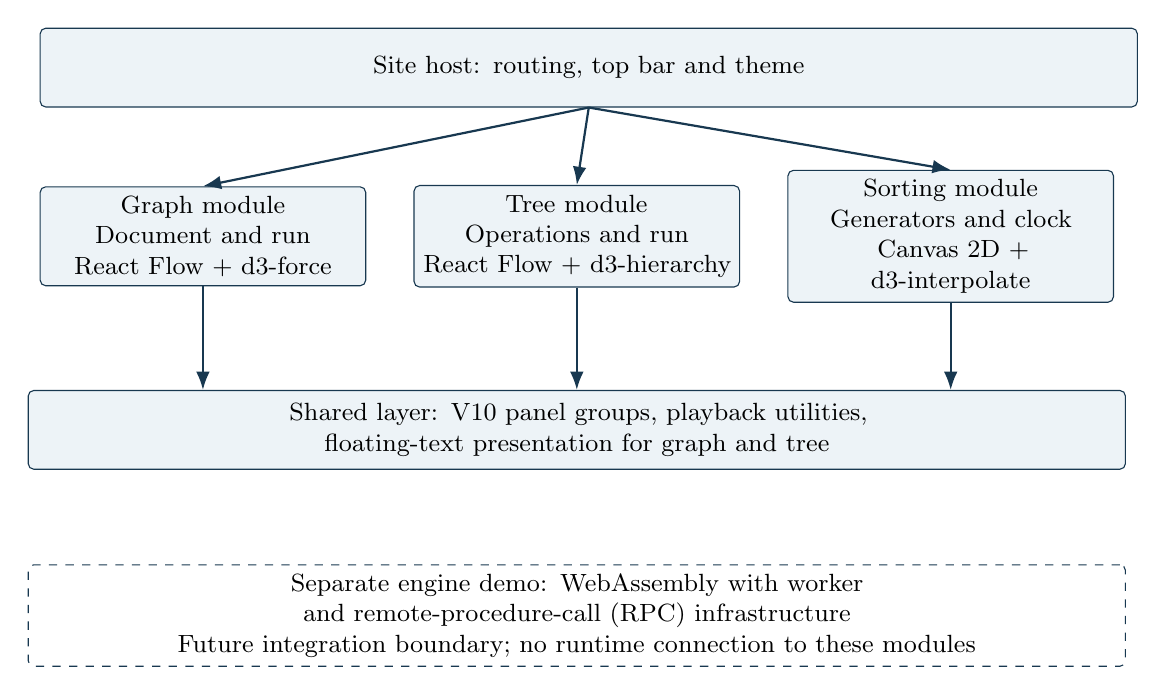
\begin{tikzpicture}[font=\small,>=Latex,
 box/.style={draw=navy,rounded corners=2pt,fill=lightblue,align=center,minimum height=10mm,text width=39mm},
 wide/.style={box,text width=137mm}, arr/.style={->,thick,draw=navy}]
\node[wide] (host) {Site host: routing, top bar and theme};
\node[box,below=10mm of host,xshift=-49mm] (g) {Graph module\\Document and run\\React Flow + d3-force};
\node[box,right=6mm of g] (t) {Tree module\\Operations and run\\React Flow + d3-hierarchy};
\node[box,right=6mm of t] (s) {Sorting module\\Generators and clock\\Canvas 2D + d3-interpolate};
\draw[arr] (host.south) -- (g.north);\draw[arr] (host.south) -- (t.north);\draw[arr] (host.south) -- (s.north);
\node[wide,below=13mm of t] (shared) {Shared layer: V10 panel groups, playback utilities,\\floating-text presentation for graph and tree};
\draw[arr] (g.south) -- (shared.north -| g.south);
\draw[arr] (t.south) -- (shared.north);
\draw[arr] (s.south) -- (shared.north -| s.south);
\node[wide,below=12mm of shared,fill=white,dashed] (wasm) {Separate engine demo: WebAssembly with worker and remote-procedure-call (RPC) infrastructure\\Future integration boundary; no runtime connection to these modules};
\end{tikzpicture}
\caption{Current application boundaries. Each module renders its own drawing; the lower dashed box is a separate prototype, not a dependency of the visualization application.}\label{fig:arch}
\end{figure}

This organization avoids making the shared shell responsible for algorithm logic. For example, the shell positions a Status panel, but the active algorithm determines its content. State is held in the browser; saved V10 layouts are versioned in local storage.

\page
\subsection{State ownership and reproducible playback}\label{sec:state}
The graph foundation separates four concerns (Table~\ref{tab:state}). A persistent canvas is reused for editing and execution. Starting a run derives a sequence of typed steps (shown as frames) from the current document; stepping through that sequence derives the visible presentation. This reduces the risk of keeping a separate editing graph and animation graph that gradually disagree.

\begin{table}[tbp]\small\centering
\caption{State separation in the graph visualizer.}\label{tab:state}
\begin{tabularx}{\linewidth}{@{}p{31mm}X X@{}}\toprule
State owner & Responsibility & Example consequence\\\midrule
Graph document & Vertices, edges, weights, stable identities and topology revision. & A semantic edit changes the topology revision, so the previous run is discarded.\\
Graph layout & Positions and pinned vertices. & Dragging a vertex changes the drawing without changing the algorithm input.\\
Run session & Step sequence, current index, run identity and playback status. & An outdated timer event cannot advance a newer run.\\
Presentation & Highlights, badges and derived edge/node styles. & Rewinding restores the presentation of the selected step.\\\bottomrule
\end{tabularx}
\end{table}

For example, moving vertex B should not change a shortest-path computation. Changing an edge weight should. Keeping position data separate from semantic input makes this distinction explicit. A run identity also protects against asynchronous playback events that arrive after the user stops or replaces a run.

Graph and tree algorithms build their complete step sequence when a run starts. The session then moves between idle, paused, playing and finished states. Each selected step supplies consistent information for the drawing, pseudocode highlight and status text. This eager approach makes backward stepping and seeking straightforward, but increases startup time and memory use for long runs. These costs have not yet been benchmarked.

Tree operations add a distinction between a preview and a committed document. An insertion or deletion can be explored through intermediate states before its final result is applied. This lets the learner inspect an operation without treating every animation frame as a permanent edit.

\subsection{Sorting uses a different execution model}
Sorting produces operations from generators. A shared clock advances one, two or four panes, each with its own operation stream. The implementation retains executed history, buffers up to 2,048 future operations, and initially primes streams up to a 60,000-operation aggregate threshold before continuing lazily. Seeking backwards reconstructs the state from retained operations; it does not rely on stored checkpoints.

This approach avoids requiring every sort to finish generating before interaction begins. However, retained history is never trimmed (only the 240-value input cap bounds it), and a backward seek replays operations from the start to the target, so its cost grows with how late the target lies. Both are limitations for future measurement. A common operation index supports synchronized inspection, but operations from different algorithms are not equivalent units of computational cost.

\page
\subsection{V10: a shared panel-group layout}\label{sec:v10}
The V10 shell organizes supporting information around a fixed central canvas. The canvas cannot become a tab. Left, right and bottom regions contain groups of tabs; a user can move a panel into a group, split it off into a new group or place it in an empty region. The default arrangement puts Action and e-Lecture on the left, with Pseudocode and Status on the right (Figure~\ref{fig:v10}).

\begin{figure}[tbp]\centering
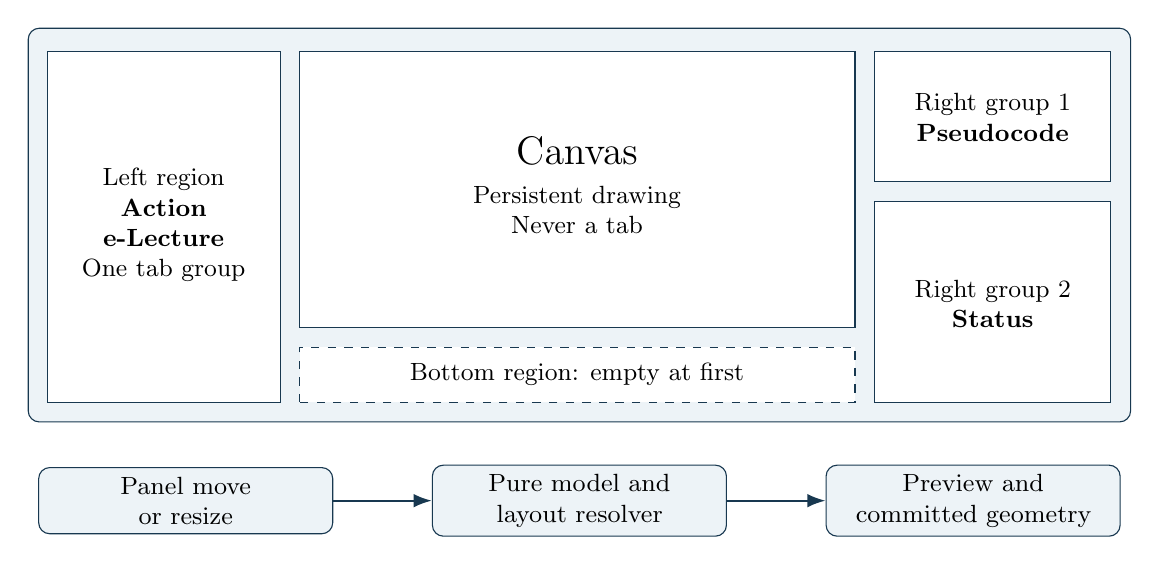
\begin{tikzpicture}[font=\small,>=Latex]
\draw[draw=navy,fill=lightblue,rounded corners] (0,0) rectangle (14,5.0);
\draw[fill=white,draw=navy] (.25,.25) rectangle (3.2,4.7);
\node[align=center] at (1.72,2.5) {Left region\\\textbf{Action}\\\textbf{e-Lecture}\\One tab group};
\draw[fill=white,draw=navy] (3.45,1.2) rectangle (10.5,4.7);
\node[align=center] at (6.97,3.0) {\Large Canvas\\[3pt]Persistent drawing\\Never a tab};
\draw[fill=white,draw=navy] (10.75,3.05) rectangle (13.75,4.7);
\node[align=center] at (12.25,3.87) {Right group 1\\\textbf{Pseudocode}};
\draw[fill=white,draw=navy] (10.75,.25) rectangle (13.75,2.8);
\node[align=center] at (12.25,1.5) {Right group 2\\\textbf{Status}};
\draw[fill=white,draw=navy,dashed] (3.45,.25) rectangle (10.5,.95);
\node at (6.97,.6) {Bottom region: empty at first};
\node[draw=navy,fill=lightblue,rounded corners,align=center,text width=35mm] (a) at (2,-1.0) {Panel move\\or resize};
\node[draw=navy,fill=lightblue,rounded corners,align=center,text width=35mm] (b) at (7,-1.0) {Pure model and\\layout resolver};
\node[draw=navy,fill=lightblue,rounded corners,align=center,text width=35mm] (c) at (12,-1.0) {Preview and\\committed geometry};
\draw[->,thick,navy] (a)--(b);\draw[->,thick,navy] (b)--(c);
\end{tikzpicture}
\caption{V10 layout and shared geometry calculation. The bottom region is shown as a target area; it does not reserve this height when empty.}\label{fig:v10}
\end{figure}

The main engineering decision was to express layout changes in a pure model rather than embedding all rules inside pointer-event handlers. The model preserves panel membership, removes empty groups and ensures that each group's active tab belongs to that group. Required panels occur exactly once, optional panels at most once, and groups do not nest.

A common layout resolver is used for sizing, target validity and drag previews. A proposed move is first represented in the model and then resolved into geometry, so the preview and committed result use the same constraints. Expanded groups keep at least 240 pixels of width and 120 pixels of height. Each module sets its own drawing floor (360 by 320 pixels for the graph; 320 by 200 or 320 by 240 pixels for tree workspaces), which the resolver keeps when the viewport can accommodate it.

Saved layouts are versioned and repaired or replaced with defaults when invalid. Automated tests and manual checks were used to verify the layout behaviour: model tests run 4,000 seeded random operations across several viewport sizes with repeated serialization round trips; browser tests move tabs through the tab menu and drag a column splitter; and the graph and tree manual checklists cover tab drag, split and splitter resizing.

\page
\subsection{The shared shell in use}
\shot{F2-dfsbfs-bfs-frame8.png}{.78}{BFS at frame 8 of 22 in the default V10 arrangement. The drawing, pseudocode, Status panel and footer playback controls refer to the same selected step.}{fig:bfs}
\shot{F3-tab-drag-preview.png}{.78}{Dragging the Action tab onto the Pseudocode group shows the proposed drop area. This screenshot records the preview, not a completed drop.}{fig:drag}

Figures~\ref{fig:bfs} and~\ref{fig:drag} show why layout is part of algorithm interaction. A learner may need more space for pseudocode while tracing a run, then more space for input editing. A common shell permits this adjustment without changing the underlying algorithm state. The same design is used across the three visualizer families.

\page
\subsection{Graph extensions and algorithm validation}
The current graph module contains 11 algorithms, counting recursive and stack-based depth-first search (DFS) separately. Alongside breadth-first search (BFS), stack-based DFS, Dijkstra, Kruskal and Edmonds--Karp, the application supports recursive DFS, Bellman--Ford, Prim, topological sorting, bipartite checking, and cut-vertex/bridge detection. Topological sorting offers DFS and Kahn methods; bipartite checking offers DFS and BFS methods. BFS, Dijkstra and Bellman--Ford also accept an optional End node; their last frame then draws the shortest path to it.

These additions extend both computation and explanation. Recursive DFS exposes a different execution structure from a stack-based traversal. Topological sorting and bipartite checking provide witnesses when the input violates their conditions, rather than displaying only a final success or failure. Bellman--Ford and Prim were planned and built with Codex under my requirements and review.

\shot{F8-cut-vertex-bridge-cp4-4-7-last.png}{.90}{Final frame of cut-vertex and bridge detection on VisuAlgo's example graph labelled CP4 4.7: the result reports cut vertices 1, 3 and 4 and bridges 0--1 and 3--4.}{fig:cut}

\textbf{A representative correctness issue: parallel edges.} A low-link DFS must skip the parent \emph{edge}, not every edge leading to the parent vertex. If two vertices are joined by two parallel edges, removing either edge leaves them connected. Ignoring both edges during DFS can incorrectly mark one as a bridge. Stable edge identities make the intended rule explicit; Figure~\ref{fig:cut} shows the detector's final result on one of VisuAlgo's example graphs.

For validation, the tests compare results with independently formulated oracles. Cut vertices and bridges are checked by removing a vertex or edge and recomputing connected components. Bellman--Ford is checked against Floyd--Warshall-based results, including negative-cycle reachability. Prim is compared with exhaustive forest candidates on small inputs. These oracles are algorithmically different from the implementations under test; this reduces shared assumptions, but is not a formal proof.

The recorded randomized cases include 700 random multigraphs for cut vertices and bridges (400 compared with the removal oracle and 300 checking the DFS-root rule), 140 signed graphs for Bellman--Ford, and 20 small graphs for Prim tested from every start vertex. Topological and bipartite methods have additional randomized checks. Fixed seeds make failures reproducible.

\page
\subsection{Tree operations and sorting comparison}
The tree visualizer provides seven workspaces: lowest common ancestor (LCA), binary search tree (BST), AVL tree, binary heap, trie, segment tree and lazy segment tree. Work includes BST/AVL queries and traversals, AVL deletion, heap operations, and lazy range-add/range-sum behaviour. The heap links array and tree representations; intermediate changes remain previews until applied (Figure~\ref{fig:heap}). These workspaces do not imply complete operation parity with VisuAlgo.

\shot{F6-heap-insert-climb-note.png}{.72}{Heap insertion of 1, frame 3 of 9: the new item at index 10 is compared with its parent 7 at index 5. The floating-text note ``$1<7$ $\cdot$ swap up'' (Section~\ref{sec:notes}) states the decision before the swap, and the array strip marks the same two items.}{fig:heap}

Sorting provides eight algorithms in a one-pane Study mode and two- or four-pane Compare mode. Panes share the input dataset and clock, making it possible to inspect different operation sequences on the same data (Figure~\ref{fig:sorting}). Duplicate algorithm selection is prevented and randomized quicksort uses a reproducible seed.

\shot{F7-sorting-compare-4-panes.png}{.72}{Four-pane comparison of Merge, Bubble, Quick and Radix sort on the same 48-element input. The shared operation index is a playback coordinate, not a measurement of relative runtime.}{fig:sorting}



\page
\subsection{Floating text: explanations on the canvas}\label{sec:notes}
A step can be meaningful even when the drawing hardly changes. For example, Dijkstra may reject a relaxation because the candidate distance is not shorter than the existing one. If the reason appears only in a separate Status panel, the learner must repeatedly look away from the relevant edge. After the Week 10 trial, I introduced floating text: short step notes placed on the canvas over the relevant node (for Dijkstra, the vertex that the relaxed edge reaches). It was one of several post-trial refinements (Section~\ref{sec:trial}) and is intended to reduce how often users look at Status while following a run, keeping their attention on the canvas. Status remains available for persistent detail; reduced attention switching is a design aim, not a measured result.

\shot{F4-sssp-dijkstra-frame24-note.png}{.94}{Dijkstra relaxation from B to E: the note explains that $4+3<8$, so E's distance changes from 8 to 7.}{fig:notes}

Figure~\ref{fig:notes} shows an accepted update. Each relaxation writes one note over its target: green when the distance changes, as here, and red when it is kept, for example ``already settled''. The implementation has a shared note description, placement calculation, timing logic and rendering layer. Graph and tree algorithms supply the semantic content; the shared layer controls how it is displayed. Current coverage includes Dijkstra, LCA, BST, AVL and Heap. Sorting, Trie, segment trees and the other graph algorithms do not yet use this layer.

Notes are rendered outside the zoom transform of the graph or tree canvas, so their text keeps a constant screen size while each note follows its node. Placement checks nearby obstacles, including node badges and edge-weight labels. It first tries preferred positions, then alternatives; when none is clear, it uses a minimum-overlap fallback. Dense graphs can therefore still produce overlap.

Timing adapts to playback. A note appears only when a step is reached by moving one step forward (Next or autoplay). After Next it lasts 1,600 milliseconds; during autoplay it is shortened to 90\% of the step interval and omitted when less than 200 milliseconds would remain, so fast playback does not accumulate unreadable text.

Because viewing alone has rarely improved learning~\cite{hundhausen2002}, the notes will be evaluated through active tasks (Table~\ref{tab:tasks}). The note layer is currently hidden from accessibility APIs, and the application has not undergone a systematic accessibility evaluation. Future work should check whether the equivalent text in Status is sufficient and whether users can understand rejected actions, rapid transitions and dense cases without relying on colour or motion alone.

\par\vspace{6pt}
\section{Current Results and Validation}\label{sec:results}
The current build provides one site with runnable graph, tree and sorting modules (Figure~\ref{fig:home}). Of its 30 catalogue cards, 12 open a module and 18 are marked coming soon. Of the 26 cards transcribed from visualgo.net's module list, eight open: four offer every algorithm the original module lists (Sorting, BST/AVL, Binary Heap and Minimum Spanning Tree) and four offer some of them (Segment Tree, Graph Traversal, Single-Source Shortest Paths and Max Flow). The other four open cards are Trie and LCA, which visualgo.net has as separate pages, and this project's own Graph and Tree Editors. These labels count algorithms, not operations.

\shot{F1-home-catalogue.png}{.66}{Top of the home page of the integrated application. Its credit line states that the site is adapted from visualgo.net; the module catalogue, including the coming-soon cards, continues below.}{fig:home}

\begin{table}[tbp]\centering\small
\caption{Recorded checks on 1 November 2026 at application commit \code{662e7b3}~\cite{validation}.}\label{tab:tests}
\begin{tabularx}{\linewidth}{@{}XrX@{}}\toprule
Check & Result & Interpretation\\\midrule
Graph unit tests & 654 passed & Algorithms, state and graph behaviour.\\
Tree unit tests & 1,881 passed & Operations, state and presentation.\\
Sorting unit tests & 571 passed & Operation streams and playback.\\
Shared / site unit tests & 143 / 24 passed & Common components and site logic.\\
\textbf{Total unit tests} & \textbf{3,273 passed} & Recorded suite total.\\
Browser cases & 151 passed & 14 test files, run in Chromium.\\
Type check / build & Passed & Compile-time and production build checks.\\
Lint & 0 errors & Two warnings remained.\\\bottomrule
\end{tabularx}
\end{table}

The recorded environment was Windows 11, Node 24.17.0, npm 11.13 and Playwright 1.64.1 with Chromium. The build emitted a large-chunk warning (about 705 kB before gzip and 206 kB after). From 4 September to 30 October, the repository's CI recorded 266 workflow runs, 105 of them in the visualizer workflows and the rest in Kerk's engine CI and the site deployment; eight failed, each followed by a passing run of the same workflow.

Passing tests support regression confidence within the tested cases (Table~\ref{tab:tests}); they do not measure usability, accessibility, browser portability or learning. Automated tests and manual checks were used to verify interface behaviour (Section~\ref{sec:v10}). The Week 10 trial provided formative feedback on usability (Section~\ref{sec:trial}).

\page
\section{User Evaluation, Limitations and Next Steps}
\subsection{Week 10 formative user trial}\label{sec:trial}
In Week 10, Kerk and I invited several users, all NUS students, to use VisuAlgo+ with the V10 layout independently for 15--20 minutes. Participants varied in prior use of VisuAlgo, from frequent to infrequent users, and in algorithm experience, from experienced competitive programmers to beginners. We recorded each session on video, administered a short test afterwards and collected feedback. Kerk asked participants in advance for permission to record and use the videos, and all agreed; the recordings show only the screen and hand interactions, not faces.

The sessions yielded positive feedback as well as areas needing improvement. Reviewing the recordings helped us identify interactions that supported familiarization with the new interface and places needing refinement. This led to several UI/UX refinements: floating text, which keeps explanations close to the visualization (Section~\ref{sec:notes}), and adjustments to the legend and Status panel.

\subsection{Evaluation and implementation limits}
Participant numbers, test questions, scores and detailed observations from the trial have not yet been compiled, so this report does not quote them. The trial provides formative design input; a post-use test alone does not establish learning gains or comparative usability, and the effect of floating text has not been measured. Performance benchmarks and a test-coverage percentage are also unavailable.

Several implementation limits are material. Graph and tree step sequences are built eagerly. Sorting keeps all history and replays it to seek backwards. Floating text covers only selected algorithms and may overlap in dense drawings. Browser validation is concentrated on desktop Chromium; mobile behaviour, cross-browser compatibility and accessibility remain incomplete. The manual developer checklists (20, 10 and 26 items for graph, sorting and tree) were run, but their runs were not recorded.

The separate engine is also a scope boundary. My unmerged experiment on Kerk's engine explored stable edge identity and a reusable browser client for worker/RPC lifecycle management. It helped identify integration requirements, but it is not part of the deployed visualizer path.

\subsection{Proposed follow-up evaluation}
I will first organize the Week 10 footage, test responses and feedback into anonymized observations linked to design changes, then conduct a more structured follow-up (Table~\ref{tab:tasks}), provisionally involving 6--10 students familiar with introductory data structures. The participant plan, consent procedure and any NUS ethics review requirement will be confirmed with the supervisor before recruitment. A small study can identify interaction problems; it cannot establish general learning effectiveness.

\begin{table}[tbp]\small\centering
\caption{Proposed tasks for the structured follow-up evaluation.}\label{tab:tasks}
\begin{tabularx}{\linewidth}{@{}>{\raggedright\arraybackslash}p{41mm}X@{}}\toprule
Task & Evidence to collect\\\midrule
Explain a Dijkstra relaxation & Correct explanation of an accepted and rejected update; use of notes, pseudocode and Status.\\
Trace heap insertion & Correct prediction of the next swap and understanding of preview versus Apply.\\
Rearrange the workspace & Successful tab move/split, recovery from an unwanted layout, errors and assistance needed.\\
Compare two sorting runs & Ability to explain an operation difference without treating operation index as elapsed runtime.\\\bottomrule
\end{tabularx}
\end{table}

Each session will record task completion, time, errors, requests for help and short participant comments; any comparison with the original VisuAlgo will use matched tasks and inputs in counterbalanced order.

\subsection{Proposed technical measurements}
Measurements will use a fixed machine and production build with saved inputs of increasing size, covering run preparation, time to first visible step, seek latency, playback frame pacing and memory use. Each condition will be repeated at least five times, and the median reported with the spread and environment. These measurements should guide whether checkpointing, bounded history or a different execution boundary is necessary.

\par\vspace{6pt}
\section{Plan for the Remaining Project}\label{sec:plan}
The agreed direction for Semester 2 is to move from prototypes to one complete web application, merging the visualizers with the shared infrastructure. Table~\ref{tab:plan} proposes milestones for this, for discussion with the supervisor and Kerk. The SoC dates are the CA presentation in Reading Week (14--20 November 2026), the final report by 5 pm on Wednesday 7 April 2027, and the final presentation on 19--23 April 2027 (tentative); the other windows are proposals.

\begin{table}[tbp]\small\centering
\caption{Proposed milestones and completion evidence.}\label{tab:plan}
\begin{tabularx}{\linewidth}{@{}>{\raggedright\arraybackslash}p{20mm}>{\raggedright\arraybackslash}X>{\raggedright\arraybackslash}X@{}}\toprule
Window & Main work & Completion evidence\\\midrule
Nov--Dec 2026 & CA presentation; consolidate Week 10 findings; stabilize the build; define follow-up tasks; keep automated and manual UI checks current. & Reproducible baseline, updated UI tests and checklists, and reviewed evaluation protocol.\\
January 2027 & Begin merging the visualizers into the complete web application with Kerk; first slice: one graph algorithm through the shared infrastructure and engine. & Written input/step contract; matching results and playback semantics against the TypeScript reference.\\
February & Conduct follow-up task evaluation and technical measurements. & Anonymized observations, fixed benchmark inputs, environment and result tables.\\
March & Address high-impact findings; improve explanation and accessibility for selected modules; consolidate results and draft the final report. & Before/after regression checks, follow-up verification of the changed tasks, and a complete report draft.\\
April & Submit the final report by 7 April; final presentation and demonstration (19--23 April, tentative); e-copy by 10 May. & Reproducible release snapshot, final evaluation account and presentation materials.\\\bottomrule
\end{tabularx}
\end{table}

\subsection{Integration strategy and risks}
Integration into the complete application should begin with one vertical slice: graph input, engine execution, typed step conversion, rendering and backward/forward playback. The first milestone is behavioural agreement, including edge identities and cancellation, rather than replacing every TypeScript algorithm. If the engine contract or schedule is not ready, the existing implementation remains a functional baseline and the final report can document the integration study separately.

The main technical risks are the cost of long step sequences, inconsistent semantics between modules, and interaction failures that model tests do not expose. Measurements should precede a major playback redesign. Shared abstractions should be introduced only where behaviour is truly common; graph/tree eager sequences and sorting generators already demonstrate that identical controls need not imply identical execution internals.

The main project risk is scope growth. Adding every unfinished catalogue topic would reduce time for evaluation and refinement. I propose prioritizing the current graph, tree and sorting workflows, selected explanation gaps and the first integration slice. Further features should be chosen with the supervisor according to educational value, missing coverage and available time.

\subsection{Expected outcome}
By the final assessment, the intended outcome is a documented and tested visualization foundation with a coherent interface, representative algorithm coverage, evidence from user tasks and technical measurements, and a clear account of progress in merging the visualizers into the complete web application. The first-semester work establishes the implementation base.

\page
\begingroup
\small
\setlength{\parskip}{3pt}
\bibliographystyle{plain}
\bibliography{references}
\endgroup
\noindent{\footnotesize Project records~\cite{evidence,architecture,validation} are the author's working records, not research publications. Screenshots show application commit \code{662e7b3}; diagrams were drawn for this report. VisuAlgo remains the source of the original educational material and examples.\par}
\end{document}
